\documentclass{article}
\usepackage[hidelinks]{hyperref}
\usepackage{graphicx}
\usepackage{amsfonts}
\usepackage{amsmath}
\usepackage{enumitem}
\usepackage{polski}
\usepackage[utf8]{inputenc}
\usepackage{indentfirst}
\usepackage{float}
\title{Projekt aplikacji do ekstremalnego uczenia maszynowego do klasyfikacji big data}
\author{Abdelkarim Ahmed, Hernik Aleksandra}
\begin{document}
Wydział Matematyki i Nauk Informacyjnych Politechniki Warszawskiej
\begin{figure}[H]
\begin{center}

\includegraphics[scale=0.5]{MiNI.png}
\end{center}
\end{figure}
\vspace*{\fill}
\begin{center}
\begin{minipage}{.9\textwidth}
\maketitle
\begin{center}Wersja 1.2\end{center}
\end{minipage}
\end{center}
\vfill % equivalent to \vspace{\fill}
\clearpage
\noindent
\begin{table}[H]
\caption{Zmiany w dokumentacji}
\hspace*{-1cm}
\begin{tabular}{|l|l|l|r|}
\hline
\textbf{Data} & \textbf{Autor} & \textbf{Opis zmian} & \textbf{Wersja} \\
\hline
10.10.2016 & Ahmed Abdelkarim & Diagram przypadków użycia & 0.1 \\
10.10.2016 & Aleksandra Hernik & Wstępna wersja harmonogramu i wymagań & 0.2 \\
19.10.2016 & Aleksandra Hernik & Korekty harmonogramu i wymagań & 0.3 \\
02.11.2016 & Ahmed Abdelkarim & Stworzenie i wprowadzenie szablonu & 1.0 \\
02.11.2016 & Ahmed Abdelkarim & Opis przypadków użycia & 1.1 \\
02.11.2016 & Aleksandra Hernik & Opis biznesowy, dokończenie harmonogramu & 1.2 \\
\hline
\end{tabular}
\end{table}
\tableofcontents
\clearpage
\section{Specyfikacja}
\subsection{Opis biznesowy}
Projekt polega na przygotowaniu dwóch aplikacji. Pierwsza jest napisana w języku Python. Druga została stworzona w środowisku Matlab. Celem obu jest przetestowanie nowego modelu sieci neuronowych - Extreme Learning Machine. Programy zapewniają możliwość wytrenowania sieci neuronowej przy użyciu różnych danych i dostarczają informacje, dotyczące czasu trwania i jakości treningu. Dzięki temu będzie możliwe określenie, czy metoda ELM może być uważana za dobrą alternatywę dla tradycyjnych architektur sieci neuronowych, a także w jakich obszarach sprawdzi się najlepiej. Szczególny nacisk został położony na zbadanie działania dla Big Data.
\subsection{Wymagania funkcjonalne}
\begin{itemize}
\item Przygotowanie danych trenujących i testowych w formie plików csv
\item Trenowanie sieci neuronowej o architekturze ELM
\item Klasyfikacja danych testowych przez wytrenowaną sieć
\item Porównywanie wyników klasyfikacji do spodziewanych rezultatów
\item Analiza jakości klasyfikacji i  czasu trwania treningu
\item Interfejs graficzny
\end{itemize}
Poniższy diagram UML przedstawia zbiór przypadków użycia aplikacji z punktu widzenia użytkownika i systemu. Dotyczy obu aplikacji.
\begin{figure}[H]
\hspace*{-1.5cm}
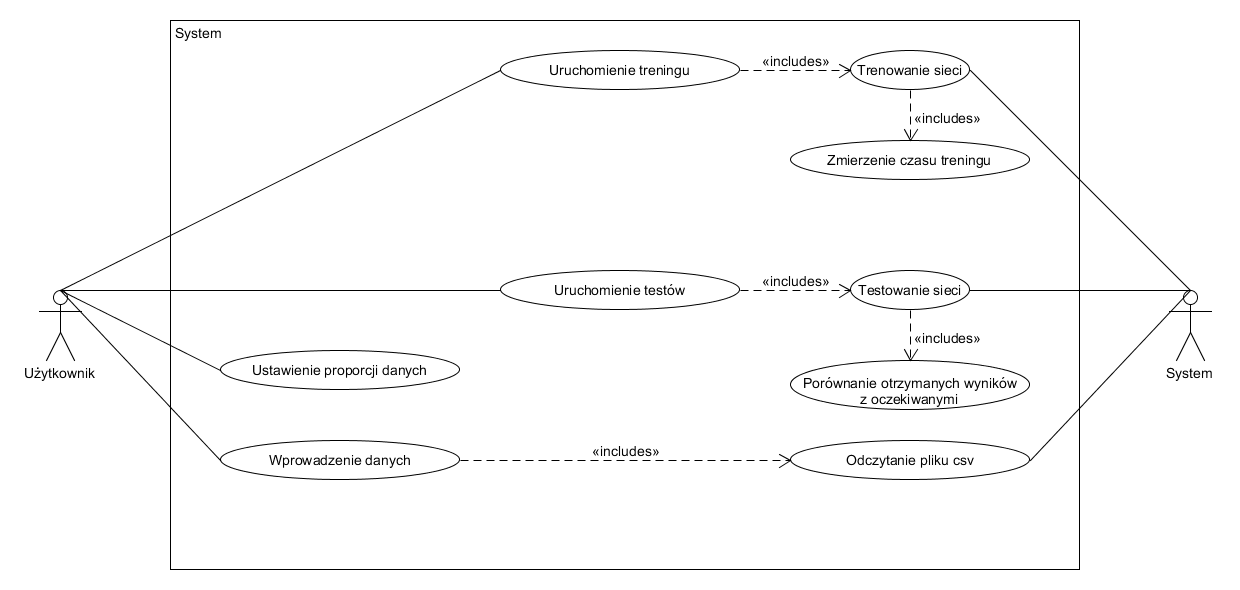
\includegraphics[width=16cm]{use_case.png}
\caption{Diagram przypadków użycia}
\end{figure}
Poniższa tabela zawiera opisy przypadków użycia dla użytkownika oraz odpowiedzi systemu.

\begin{table}[H]
\caption{Opisy przypadków użycia}
\begin{tabular}{|p{3.4cm}|p{5cm}|p{4cm}|}
\hline
\textbf{Nazwa} & \textbf{Opis} & \textbf{Odpowiedź systemu} \\
\hline
Wprowadzenie danych & Wprowadzenie danych używanych do uczenia sieci & Odczytanie pliku csv \\ \hline
Ustawienie proporcji danych & Ustawienie proporcji danych treningowych, testowych i zatwierdzających & Zapisanie wyboru \\ \hline
Uruchomienie treningu & Uruchomienie treningu sieci schematem ELM & Trenowanie sieci i zmierzenie czasu treningu \\ \hline
Uruchomienie testów & Uruchomienie testów sieci wytrenowanej wcześniej schematem ELM & Testowanie sieci i porównanie otrzymanych wyników z oczekiwanymi \\
\hline
\end{tabular}
\end{table}
\clearpage
\subsection{Wymagania niefunkcjonalne}
W poniższej tabeli znajduje się lista wymagań niefunkcjonalnych.
\begin{table}[H]
\caption{Lista wymagań niefunkcjonalnych}
\begin{tabular}{|l|l|p{9.4cm}|}
\hline
\textbf{Obszar} & \textbf{Numer} & \textbf{Opis} \\
\hline
Użyteczność & 1 & Aplikacje muszą działać na komputerach wydziałowych \\
 & 2 & Aplikacje powinny mieć przejrzysty interfejs graficzny \\
 & 3 & Wykresy wyświetlane w aplikacji powinny być czytelne \\
\hline
Wydajność & 4 & Działanie w oparciu o ELM powinno dawać o kilka rzędów wielkości szybszy czas uczenia niż tradycyjne metody \\
\hline 
Inne & 5 & Wykonanie aplikacji w językach Python i MATLAB \\
& 6 & Dobrze udokumentowany kod \\
\hline
\end{tabular}
\end{table}

\subsection{Harmonogram projektu}
\begin{table}[H]
\caption{Harmonogram prac}
\begin{tabular}{|l|r|r|r|}
\hline
\textbf{Etap} & \textbf{Czas} & \textbf{Początek} & \textbf{Koniec} \\
\hline
Przygotowanie pierwszego rozdziału dokumentacji & 24 dni & 10.10.2016 & 02.11.2016 \\
Opracowanie modelu pracy sieci ELM & 14 dni & 17.10.2016 & 30.10.2016 \\
Analiza narzędzi & 7 dni & 31.10.2016 & 06.11.2016 \\
Projekt techniczny & 7 dni & 07.11.2016 & 13.11.2016 \\
Implementacja i napisanie drugiego rozdziału pracy & 14 dni & 07.11.2016 & 20.11.2016 \\
Tworzenie i wykonywanie testów dla small data & 7 dni & 21.11.2016 & 27.11.2016 \\
Tworzenie i wykonywanie testów dla big data & 7 dni & 28.11.2016 & 04.12.2016 \\
Opis wniosków z testów & 7 dni & 05.12.2016 & 11.12.2016 \\
Instrukcja użytkownika & 4 dni & 11.12.2016 & 14.12.2016 \\
\hline
\end{tabular}
\end{table}
\subsection{Uwagi}
\begin{itemize}
\item Automatyczne testy, sprawdzające główną funkcjonalność programu - trening sieci - nie zostaną utworzone. Istotą projektu jest przeanalizowanie otrzymywanych, a nie otrzymanie z góry zaplanowanych wyników.
\item Nie zostały postawione wymagania związane z niezawodnością i utrzymaniem. Aplikacje służą wyłącznie jako narzędzia do przetestowania nowej technologii, więc jedynym wymaganiem jest działanie w momencie przeprowadzania testów. Ta kwestia może ulec zmianie, jeśli testy wypadną korzystnie dla ELM.
\item Wydajność jest raczej oczekiwaniem, nie wymaganiem. Z prac, na których bazowany jest projekt wynika, że metoda powinna być szybka, jednak założenia projektu polegają na sprawdzeniu, a nie przyjęciu tej tezy. Ponadto nie zostały zaimplementowane inne metody uczenia sieci neuronowych, więc precyzyjna ocena wydajności byłaby trudna.
\end{itemize}
\clearpage
\section{Wykaz ważniejszych oznaczeń i akronimów}
\begin{itemize}[label={},leftmargin=*]
\item Big Data -- dane z liczbą próbek tak dużą, że nie występuje efekt przeuczenia
\item ELM -- \textbf{E}xtreme \textbf{L}earning \textbf{M}achine - ekstremalne uczenie maszynowe
\item Small Data -- dane, dla których jest za mało próbek, aby sieć poznała dokładnie model bez przeuczenia
\item Toolbox -- zbiór funkcji stworzonych we wspólnym celu; biblioteka;
\end{itemize}

\end{document}